%*******************************************************************************
%*********************************** First Chapter *****************************
%*******************************************************************************

\chapter{Introduction} \label{chapter1}


% **************************** Define Graphics Path **************************
%\ifpdf
%    \graphicspath{{chapter1/figs/raster/}{chapter1/figs/PDF/}{chapter1/figs/}}
%\else
%    \graphicspath{{chapter1/figs/vector/}{chapter1/figs/}}
%\fi
\graphicspath{{figs/chapter1/PDF/}}



\section{Background}
Human movement involves not only multiple
joints and limbs for a specific task in a determined environment
but also external information processed through all of our available 
senses and our prior experiences. 
Recent studies in human motion recognition have revealed the possibility 
of estimating features from lower dimension signals to distinguish 
differences between styles of movement, such as pedalling 
\citep{Quintana-Duque2012, Quintana-Duque2016} or walking 
\citep{sama2013, frank2010}. 
Similar approaches have been applied to pattern recognition of 
physiological signals (speech and heart pathologies or epilepsy) 
\citep{gomezgarcia2014}.

Signals of lower dimension are generally time series 
of one-dimension in $\mathbb{R}$ which commonly have high nonlinearity, 
complexity, and non-stationarity 
\citep{gomezgarcia2014, huffaker2017, caballero2014}.
With that in mind, traditional methods in time-domain or 
frequency-domain generally tend to fail when detecting 
tiny modulations in frequency or phase \citep{marwan2011}. 
This can mean that subtle signatures of each 
individual's movement could be missed using traditional methods. 
However, methods of nonlinear time series analysis 
can quantify such subtleties in human movement variability 
\citep{Quintana-Duque2012, Quintana-Duque2016, sama2013, 
frank2010, gomezgarcia2014, marwan2011, stergiou2011, packard1980}.
Recently, \cite{bradley2015} reviewed methods for
nonlinear time series analysis, such as the reconstructed state space 
(RSS) \citep{takens1981}, recurrence plots (RP) \citep{eckmann1987} and
recurrence quantification analysis (RQA) \citep{zbilut1992}.
Such methods are implemented using embedding parameters ($m$ and $\tau$).
However, the computation of embedding parameters is still an open problem
since there is no general technique to compute the embedding parameters 
because time series are system-dependent, meaning that defined parameters
may only work for one purpose, e.g., prediction, or may not work well 
for other purposes e.g., computing dynamical invariants \citep{bradley2015}.

In addition, the quality of the time series signals is reflected on 
the reliability of the results for nonlinear tools. For instance, 
methodologies to compute embedding 
parameters e.g., autocorrelation, mutual information, and nearest neighbour,
require data which are well sampled and with little noise \citep{garland2016} 
or need to be purely deterministic signals \citep{kantz2003}.
Similarly, methods such as RSS, RP and RQA can break down when 
datasets have different length, different accuracy and 
precision \citep{frank2010},
%(rounding errors due to finite precision of the measurement apparatus which 
%include frequency acquisition \cite{frank2010}),
or when data are contaminated with different or unknown sources of noise 
\citep{garland2016}. It is surprising that despite these problems,
nonlinear dynamics have proven to be helpful to understand and 
to characterise time series in the context of human movement 
\citep{Quintana-Duque2012, Quintana-Duque2016, sama2013, frank2010,
gomezgarcia2014, marwan2011, stergiou2011, bradley2015}.
Another point to consider when analysing time series analysis using 
nonlinear dynamics is the appropriate use of post-processing techniques 
such as interpolation, filtering or normalisation.
However, there is little research on the effects of post-processing 
techniques and the interpretation of the results for RSSs, RPs and 
metrics of RQA.



\section{Movement Variability}
Variability is inherent within and between all biological 
systems \citep{newell1993}.
For instance, variability has been studied in electroencephalographic 
signals in human brains \citep{klonowski2007}, in physiological signals 
like the heart rate variability \citep{schumacher2004, acharya2006}, 
respiratory patterns of rats \citep{dhingra2011}, in speech variability 
where not only the linguistic aspect is investigated but 
factors like gender, age, social, state of health, emotional state are
strongly related to uniqueness of the speaker \citep{benzeghiba2007}
or even in odor responses based on cultural background and 
gender \citep{ferdenzi2013}.

Variability has also been well studied in human body movement, where, 
for instance, \cite{bernstein1967} stated that no human movement is 
repeated exactly with the same trajectory.
With that in mind, movement variability has been used as a model of fatigue 
to prevent chronic musculoskeletal disorders 
\citep{mathiassen2006, srinivasan2012}. 
Movement variability has also been considered as an indicator of skilled 
performance in sport science where, for instance, 
\cite{wagner2012} show how movement variability based on statistical 
analysis varies with skill for three levels of throwing techniques 
(low-skilled, skilled, and high-skilled).
Therefore, \cite{bartlett2007} concluded that movement variability is 
ubiquitous across sports (javelin throwing, basketball shooting or running).
Another interesting example is that movement variability can be considered 
as an identifier for personal trait \citep{sandlund2017}, 
where many factors of the human body can be considered for identification, 
such as:
age \citep{kruger2013, macdonald2006, vaillancourt2003, stergiou2016},
gender \citep{svendsen2010},
pain status \citep{madeleine2008, sandlund2008},
body composition  \citep{chiari2002},
work experience \citep{madeleine2009},
pace, movement direction or cognitive demands  
like perception, memory or capacity for introspection 
\citep{srinivasan2012, kanai2011}.
Additionally, \cite{bartlett2007} highlighted that movement variability 
can be interpreted from different theoretical disciplines.
For instance, a cognitive control theorist considers variability as 
undesirable noise and variability is reduced as skill increases, meaning 
that "becoming dexterous freezes unwanted degrees of freedom in the 
kinematic chain" \citep[p. 238]{bartlett2007}.
In contrast, an ecological motor control specialist considers movement 
variability either as a functional role in human movement for 
"coordination change and flexibility to adapt" in different 
environments \citep[p. 238]{bartlett2007} or 
as an exploration and exploitation of body parts in the 
"perceptual-motor workspace" \citep{wu2014, herzfeld2014}.

\cite{stergiou2011}, in contrast, highlighted that an optimal state 
of movement variability is associated with healthiness.
For instance, motor disabilities may be related to either 
(i) wide range of behaviours which appear to be random, unfocussed and 
unpredictable or (ii) narrow range of behaviours which seems to be rigid, 
inflexible and predictable. 
Specifically, postural sway variability which is larger for patients 
with Parkinson disease or the likelihood of falling in elderly individuals 
which is associated with too little or too much step width variability.
This suggest that extremes of movement variability are symptomatic of 
lower ability to control movement.
 

\subsection{Modelling Human Movement Variability}
Human movement involves a complex system where many sensorimotor 
variables such as joints, muscles, nervous system, motor unit and cells 
are the sources for different types of variability \citep{newell1993}.
Hence, variability encompasses different types, sources and views of 
variability.
For instance, from a biomechanical view, motion variability can be modelled
as system of differential equations for the neuro-musculoskeletal 
control system where motion variations can occur because of 
"perturbations of initial states of the skeletal system",
perturbations of "muscular or neural subsystems ",
or "external torques and forces acting on the skeletal system" 
\citep[p. 13]{hatze1986}.
According to \cite{hatze1986} motion variability can be caused by 
(i) direct consequences of adaptive learning process, and 
(ii) random fluctuations which are the result of stochastic processes 
in the nervous system. Hence, \cite{hatze1986} proposed measures of 
dispersion (e.g. Fourier series and entropy measures) to quantify the 
deviation of motion from a certain reference. With that, 
\cite{hatze1986} pointed out that the combination of deviations from 
angular coordinates (radians) and linear coordinates (meters)
for Fourier series were an unacceptable quantifier as the units are different.
Hence, \cite{hatze1986} proposed the use of entropy as a global quantifier 
for motion variability and concluded that any movement deviation of a 
body joint may be the result of deterministic and stochastic causes.




Another approach to model variability has been proposed by \cite{muller2004},
who decompose variability into exploration of 
task tolerance($T$), noise reduction($N$), and covariation($C$).
Hence, the quality of performance in 
goal-oriented tasks, 
e.g. hitting a target, is defined "by the accuracy and replicability of the 
results" (deviations from the target) "over repeated attempts of execution" 
(configuration of joint angles with its velocity, angles and position)
\citep[p. 229]{muller2004}.
For the experiment, \cite{muller2004} considered table skittles, 
where participants throw a ball on a string that swings around 
a center post with the objective of knocking down the skittle at the 
opposite site.
Then, \cite{muller2004} proposed $D$ as the absolute average of distance to
the targets in $n$ trials and used this as a measure of the collective 
performance that combines a function for movement based on the 
execution vector with a function for the minimum distance from the target $d$.
Therefore, the overall difference in performance $D$ is decomposed
into three unequal contributions of covariation $C$, 
noise reduction $N$ and task tolerance $T$.
Considering a 2-D task space that spanned the release angle $\alpha$
and absolute velocity $v$, the components of contributions of
variability were calculated from five data sets 
($A$, $A_0$, $A_{shift}$, $B$ and $B_0$):
(i) the component of covariation where sets $A$ and $A_0$ and $B$ and $B_0$ 
have the same means and variances,
(ii) the component of tolerance where sets $A$ and $A_{shift}$ differ only on
their location in the task space, and 
(iii) the component of noise where sets $A_{shift}$ and $B_0$ have the same
means but different variances 
(see Fig. 6 in \cite{muller2004} for further details).
With that in mind, \cite{muller2004} conducted an experiment with 
forty-two participants for five different locations of the target 
skittle where for each target a participant performed 320 trials which is a 
total of 1600 trials and therefore presented statistical confirmation of the 
contributions of $T$, $N$ and $C$ using ANOVA. Hence, \cite{muller2004} 
concluded that $T$ and $N$ contribute more to improvement of a 
performance of a task than $C$ for initial practice, 
meaning that a new combination of angles and velocities explore a 
large region of solution space (hitting the target).
However, for later practice $T$ diminishes, and $N$ and $C$ started to 
be more relevant.
Also, \cite{muller2004} showed in various experiments of throwing actions
that variability in the movement results (deviations from the target) 
is generally smaller than variability in the execution
(variables or release angles and velocities) for which 
it is concluded that covariation between execution variables
is another component of variability.
With that in mind, \cite{muller2004} concluded that task space exploration 
is an essential  contribution to the improvement of movement performances
which is an explanation to the increase of noise in early practice phases.

\cite{seifert2011} investigated coordination profiles for recreational and 
competitive breaststroke swimmers and proposed an hourglass model of 
variability that illustrates the amount of variability as a function of 
expertise. Hence, \citealt[p. 551]{seifert2011} stated 
recreational swimmers show a considerable amount of intra-variability 
"as they seek an individually appropriate coordination pattern to accommodate
the novel constrains of locomotion in water", whereas experts swimmers, 
after a considerable practice,  
will still explore new environments to optimise their technique that 
create another secondary blooming of variability which is 
the result of "the environment exploration to optimise their technique 
with their individual strengths (e.g. physical, anatomical, mental, etc.)
and to gain an advantage over competitive swimmers".
To test the hourglass model of variability, 
\cite{seifert2011} considered the continuous relative phase (CRP) 
between the elbow phase angle and knee phase angle, therefore CRP 
is used as an indicator on how swimmers synchronise
arm recovery (elbow extension) and leg recovery (knee flexion).
\cite{seifert2011} analysed inter-individual variability of 
swimmers with the shape of the curves of CRP which provide an indication 
of the inter-limb coordination, applied statistical measures such as 
hierarchical clustering using eleven variables of CRP 
to classify the recreational swimmers into three cluster of coordination 
(intermediate, most-variable and in-phase)
and used Fisher information to test which CRP variables were significantly 
differentiated the clusters. With that, \cite{seifert2011} concluded that 
inter-individual coordination variability for recreational swimmers could be 
the result of (i) different state of process learning, (ii) environmental 
constraints (different perception of the aquatic resistance), or (iii) 
different perception of the task constrains (floating instead of swimming).

\cite{preatoni2007} and \cite{preatoni2010, preatoni2013} report  
that inter-trial variability is defined as combination of functional changes 
associated with the nonlinear properties of the neuro-musculo-skeletal 
system ($V_{nl}$) and random fluctuations in the neuro-motor-skeletal 
system ($V_e$).
Additionally, \citealt[p. 72]{preatoni2013} stated that the random fluctuations 
in movement variability can be composed by $V_{e}=V_{eb}+V_{ee}+V_{em}$,
where $V_{eb}$ relates to the behavior and is the "error in the sensory 
information and in the motor output commands",
$V_{ee}$ is the "changes in the environmental conditions" and 
$V_{em}$ is the "changes in measuring and data processing procedures".
Therefore, similar as \cite{hatze1986}, \citealt[p. 77]{preatoni2013} 
pointed out that $V_{nl}$ "may be interpreted as the flexibility of the 
system to explore different strategies to find the most effective 
strategy among the many available".
%which is also investigated by \citep{wu2014, herzfeld2014}
Hence, \citealt[p. 1328]{preatoni2010} concluded that the total variability 
represents the changes of contributions for $V_e$ and $V_{nl}$ 
and it is defined as $V_{tol}=V_e+V_{nl}$, where $V_{tol}$ 
"may reveal the effects of adaptation, pathologies and skills learning".
Also, \cite{preatoni2013} noted that their work only investigate error from 
biological variability (e.g. $V_{eb}$) which does not consider 
non-biological noise resulting from measuring instruments or 
data post-processing techniques, such 
non-biological noise has high frequency components that are usually removed.
Therefore, the work of \cite{preatoni2010} and \cite{preatoni2013} 
do not consider an overall index to quantify movement variability but 
the combination of both $V_{eb}$ and $V_{nl}$. 
With that in mind, \cite{preatoni2007} analysed the influences of 
$V_{eb}$ and $V_{nl}$ for movement repeatability by comparing entropy measures 
(e.g. ApEn and SampEn) with values of their surrogate counterparts.


Generally, the previous approaches reported different models 
for movement variability which then are quantified with different tools.
For instance, \cite{hatze1986} and \cite{preatoni2010, preatoni2013} 
use entropy measures as the authors consider that the origin of the 
signals in the human body is the result of deterministic and 
stochastic processes, whereas 
\cite{muller2004} and \cite{seifert2011} reported 
measures of magnitude that limited the evaluation of the 
whole trajectories as structures of movement variability in 
human body activities.
Therefore, for this thesis, it is important to note that
even with the proposed models for movement variability 
\citep{hatze1986, preatoni2010, preatoni2013, muller2004, seifert2011} 
which have been quantified with statistical or nonlinear tools,
little has been investigated with regards to the reliability of the nonlinear 
tools when using real-world data that is commonly noisy, 
deterministic, stochastic or nonstationary \citep{newell1998}.
A further review of nonlinear analyses is presented in Chapter \ref{chapter2}.

\subsection{Movement Variability in Human-Humanoid Interaction}
Movement variability in the context of human-humanoid interaction has been 
investigated for exercising, rehabilitation and dancing purposes in the 
last six years
\citep{gorer2013, guneysu2014, guneysu2015, tsuchida2013, peng2015}.

For instance, \cite{gorer2013} conducted an experiment of a robotic 
fitness coach 
where eight elderly participants performed five gestures: 
three for arm related exercises and two for leg strength exercises. 
Hence, \cite{gorer2013} with only graphical 
visualisation of joint angles trajectories extracted from the pose estimation
of a kinect sensor, 
stated that only one subject out of eight fail to imitate the gestures 
correctly.
Additionally,
\cite{gorer2013} surveyed 
participants using a 5-point Likert scale about the positive and 
negative effect, flow, immersion and challenge of the human-robot 
interaction activity, concluding that their system is easy to use 
based on the high scores for immersion and 
positive effect and low scores for challenge and negative effect.
However, the small sample size and somewhat naive analysis of data
in the study makes it difficult to generalise these findings.


Another example is the work of \cite{guneysu2014} who conducted experiments 
with children for upper 
arm rehabilitation using a play-like child robot interaction.
Hence, \cite{guneysu2014}, using a Kinect sensor to get data of join angles of 
the participants` skeleton, performed an automatic evaluation of three 
upper body actions (shoulder abduction, shoulder vertical flexion and 
extension, and elbow flexion) of eight healthy children who mimicked an 
humanoid robot. To evaluate motion imitation, \citealt[p. 202]{guneysu2014} 
considered similarity error using Dynamic Time Warping (DTW) that 
penalise large angle errors over ten percent in the area range of the 
motion type and applied recall measure as a representation of 
"how much of angular area of the baseline motion
from the humanoid robot is also covered by the child's motion".
%\cite[p. 202]{guneysu2014}.
Then, \cite{guneysu2014} presented the evaluation of five physiotherapists 
using Intraclass correlation coefficient (ICC) which is a metric for 
reliability of ratings for motion types, and reported that for the 
first motion, which consists of only one joint, the metric and 
physiotherapist evaluations showed high agreement, whereas for the 
second and third motions, which motions were more complicated 
consisting of more joint values, the evaluation between the metrics 
and physiotherapist ratings differed.
\citealt[p. 203]{guneysu2014} stated that during the evaluation of complicated 
movements, children misperceived the actions for which "therapists
compensated such misunderstanding by giving high scores to the children
while the proposed system only considered angles".
This suggests that it is also possible that the physiotherapist' ratings 
differed from these data because they were considering aspects 
which could have been incidental to the movements.
With that in mind, it is interesting to note that 
similarity error and recall measures with the ICC metric are not 
completely reliable since 
they did not model well complex movements.
Recently, \cite{guneysu2015} presented an improvement of their previous research
where less complex movements, from four physiotherapists performing five 
actions, were analysed: opening a door with a key, 
touching the opposite shoulder with hand, taking an object from back to neck, 
taking an object from the back and reaching an object above the head.
Then, \cite{guneysu2015} applied traditional statistics 
(e.g. sample mean and sample variance) to characterise the five actions.
For instance, the  initial positions of arms changed from person to person, 
specially for the key turning action which variation were affected by the 
sample mean, while performances of turning the amplitude of the arm
were associated with the standard deviation of the data.
However, such statistical differences cannot capture the structure of the 
time series from each of the participants which performed the movements
at different frequencies and therefore with different data length
(see Fig. 10 in \cite{guneysu2015} for further details).


Movement variability in the context of human-humanoid interaction has also been
investigated in robotic dance activities.
For example, \cite{tsuchida2013} explored four dance formations which were 
performed three times by nine participants who had three years of experience: 
dancing with a robot, dancing alone, dancing with a self-propelled robot and 
dancing with a projected video.
To visualise dance movements, \cite{tsuchida2013} presented two participant's 
movement positions with twelve trajectories each (four dance activities times 
three trials) of z and x directions obtained with a Kinect sensor.
Although, the dance experiment was rich in terms of movement variability
for both participants and dance activities, only distance between each of 
the conditions in the dance formation was considered. 
With that, \cite{tsuchida2013} concluded that the sense of dancing with a 
projected video of a person were the closest to dance with a real person and 
the trajectory of dance with a self-propelled robot were the closest 
to the trajectory of a dancer. Additionally, \cite{tsuchida2013} only applied 
traditional statistics (e.g. ANOVA) to characterise dance movements.





Another aspect of movement variability in the context of human-humanoid 
interaction is the generation of robotic dance.
Recently, \cite{peng2015} reviewed an hierarchical taxonomy of 
four categories of robotic dance (cooperative human-robot dance, 
imitation of human dance motions, synchronisation for music and 
creation of robotic choreography).
\cite{peng2015} pointed out that the creation of robotic dances is still 
an open research question because dance motions should generally be both 
interesting and exciting for users. 
According to \cite{peng2015}, the creation of robotic dances can be 
accomplished with any of the following methodologies:
(i) random generation: where robots can be 
programmed with series of predefined algorithms that can be chosen randomly,
(ii) mapping rule:  where robots can react, and therefore dance, to different 
factors such as colours, sounds, speech, temperature or human activity,
(iii) chaotic dynamics: which are sensitive to initial conditions and 
can create various dance styles from periodic and couple to rhythm to 
jumping styles, resulting in innovative and consistent dance patterns,
(iv) interactive reinforcement learning: where the robot can automatically 
choose motions based on rewards of participants' 
preferences of graceful motions,
(v) evolutionary computation: in which multiple iterations of generations
of dance motions can create graceful robotic dance motions, and
finally (vi) using a Markov chain model, a discrete time stochastic chain, 
where each sequence of dance motions is considered as a state in the Markov 
chain producing dance that synchronise with music and emotions.
Therefore, while the research questions of this thesis are not fully related 
to the creation of good robotic dances (e.g, being innovative or having 
accordance with human aesthetics) \citep{peng2015}, it is important to note 
that one of the methodologies to create robotic dance motions is the use of 
chaotic dynamics
which consider initial conditions to generate movements 
that are neither deterministic nor stochastic.

Although, movement variability in the context of human-humanoid interaction
has not been directly investigated in recent years, it can be noted 
that movement variability is indeed applied in exercise, 
rehabilitation or dance.
Hence, it can be noted that previous work that has analysed gestures, 
movements or dance activities with only traditional statistics, for which
(i) it is not clear how \cite{gorer2013} performed the evaluation of 
synchronisation for gestures between participants and the humanoid
nor what were the methods of evaluation, apart from the visual 
which had been applied to classify correct gestures trajectories,
 and (ii) little has been investigated with regards to the 
differences in movement of the invited physiotherapists in the work of
\cite{guneysu2014} and  \cite{guneysu2015},
(iii) it is not clear, in the results of \cite{tsuchida2013}, 
why the distribution of trajectories for subject 1 
were more uniform than the trajectories of subject 2, and
(iv) even though, the robot movements for the experiments of this thesis 
are simple and pre-programed, \cite{peng2015} noted that generation of 
robotic dance movements can be done with chaotic dynamics.

Therefore, it is suggested that applying nonlinear analyses 
instead of traditional statistics in the context of human-humanoid 
interaction might provide a better quantification and understanding
of human movements since these are generally both deterministic and stochastic.
Similarly, little research has been done in this context 
with regards to the reliability of nonlinear tools 
when using real-world time series 
(e.g. window length, post-processing techniques, 
noise contamination, nonstationarity, chaotic deterministic, etc).



\section{Research questions}
A number of questions regarding movement variability (MV) have been 
investigated in the last decade:
%\citep{stergiou2006, stergiou2011} such as: 
how is variability controlled 
while learning a new skill? \citep{wagner2012, seifert2011, bartlett2007}, 
is variability associated with disease or health? 
\citep{stergiou2006, stergiou2011}, what are the sources of variability 
and how do they interact in the production of observed variation 
of movement? \citep{preatoni2007, preatoni2010, preatoni2013}.
Nonetheless, little has been investigated regarding to the 
reliability of nonlinear tools to quantify movement 
variability \citep{iwanski1998, yao2017}
when dealing with real-world data \citep{bradley2015, caballero2014}.
Therefore, this thesis explores the effects on three nonlinear tools
(e.g. Reconstructed State Space (RSS), Recurrence Plots (RP) and 
Recurrence Quantification Analysis (RQA)) with different features 
of time series such as structure, levels of smoothness and window lengths.
To perform such exploration, two experiments were conducted with twenty 
right-handed healthy participants: one for human-image imitation 
activities and another in the context of human-humanoid imitation 
activities.
For the experiments, participants were asked to imitate simple arm movements
and participants and humanoid robot worn inertial sensors that collected 
time series.
Hence, three research questions are investigated in this thesis.

\begin{itemize}

\item What are the effects on RSSs, RPs, and RQA metrics
	of different embedding parameters, different recurrence thresholds 
	and different characteristics of time series 
	(window length size, smoothness and structure)?

\item Additionally, what are the weaknesses and strengths of 
	RQA metrics when quantifying MV?

\item How the smoothing of raw time series affects the nonlinear analyses
	when quantifying MV?

\end{itemize}




\newpage
\section{Outline of the thesis}
This thesis is organised as shown in Fig. \ref{fig:thesis-outline}.
Chapter 1 presents a background of quantification of 
Movement Variability(MV), state-of-the-art for modelling human MV,
MV in the context of human-humanoid interaction and research questions
are stated.
Chapter 2 presents an introduction to fundamentals of time series
analysis in terms of: (i) what to measure in Movement Variability(MV)?
and (ii) which nonlinear tools are appropriate to measure MV?, 
including a review of the state-of-the-art literature of nonlinear 
analyse with real-word data. 
It is then presented in Chapter 3 a review of state space 
reconstruction method that entails an explanation for uniform time 
delay embedding (UTDE) and a description of the techniques to estimate 
of minimum embedding parameters (e.g. false nearest neighbour and 
average mutual information), an introduction to Recurrence Plots (RPs),
structures of RPs and different metrics to perform 
Recurrence Quantification Analysis (RQA) as well as the 
weakness and strengthens of RPs and RQAs.
In Chapter 4, the experiments for human-image imitation and human-humanoid 
imitation are presented describing aims, participants, activities in the 
experiments, equipment, ethics and preparations of the time series.
Chapter 5 and 6 present the results with regards to two experiments
(human-image imitation and human-humanoid imitation) for 
minimum embedding parameters, reconstructed state space using 
uniform time-delay embedding, recurrence plots, recurrence quantification 
analysis(RQA) metrics and 3D surfaces of RQA metrics to show the
weaknesses and strengths of RQA.
Finally, Chapter 7 presents conclusions, the answers for the
research questions, the contribution to knowledge and 
future work for this thesis.

%---------------------------------(FIGURE)-------------------------------------
\begin{figure}
\centering
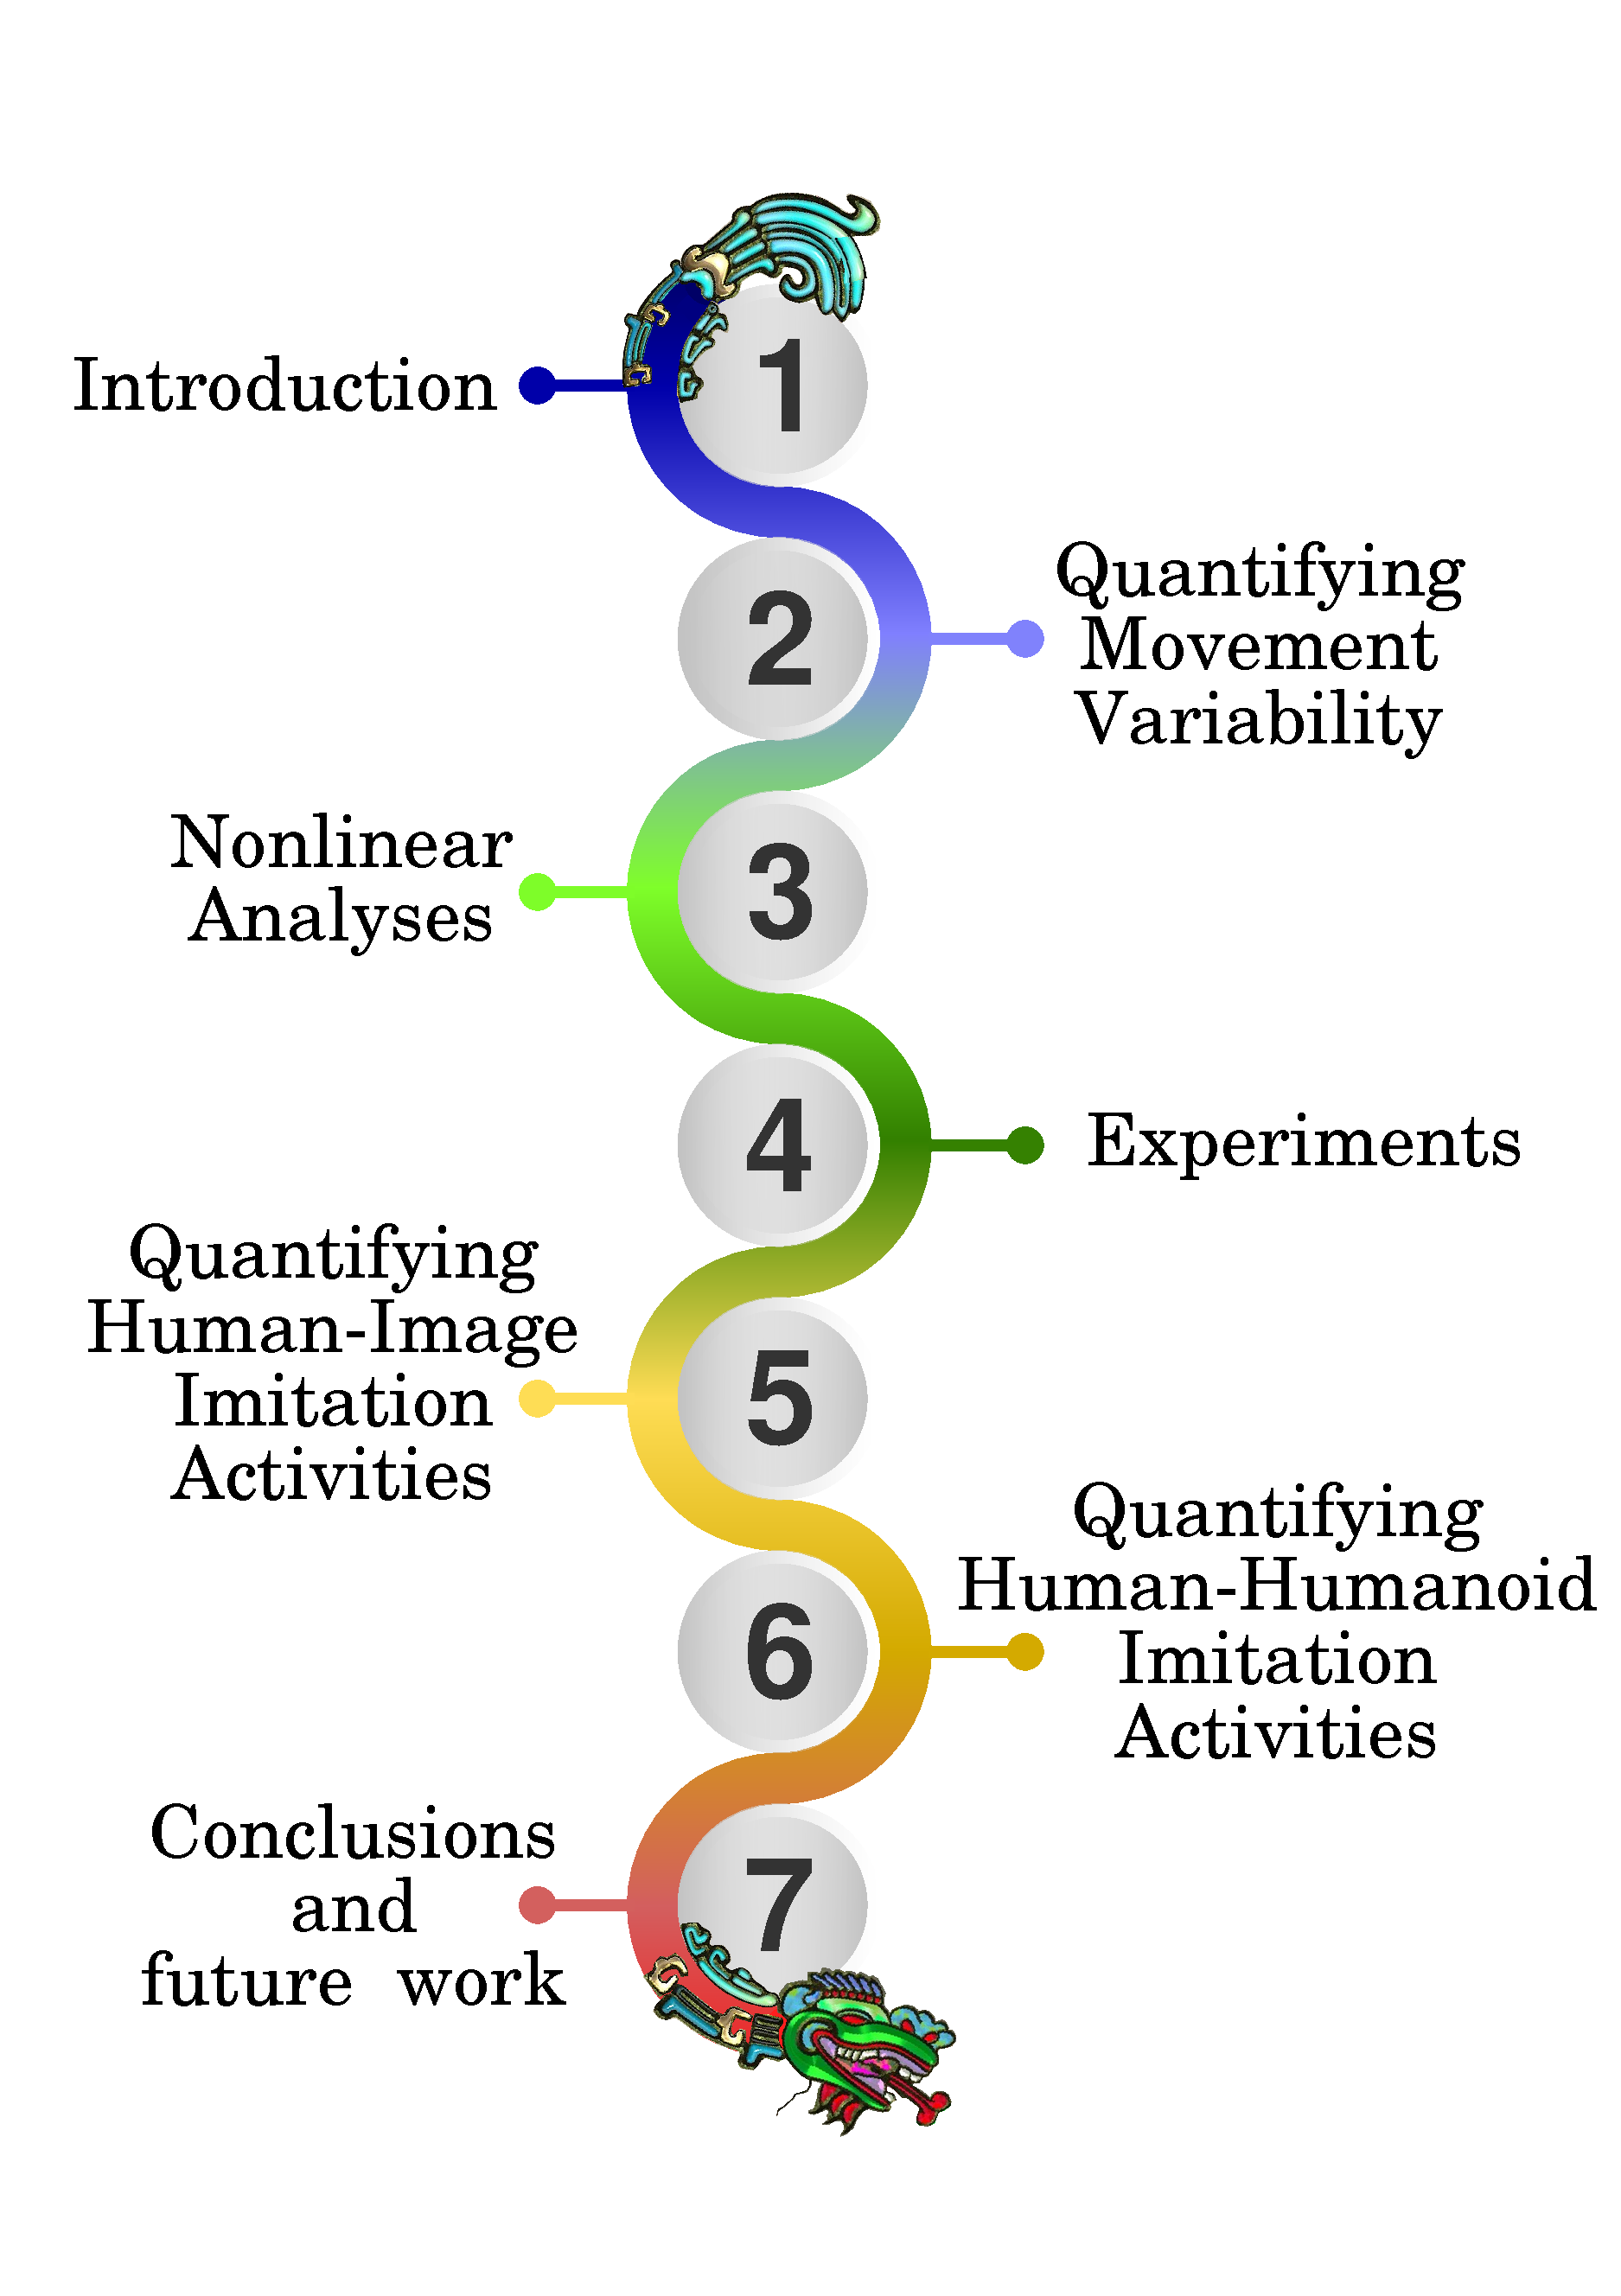
\includegraphics[width=0.92\textwidth]{toutline}
    \caption[Thesis outline]{
	{\bf Thesis outline.}
	Chapter numbers with its titles. 
	N.B. Quetzalcoalt is flowing between chapters.
	"To the Aztecs, Quetzalcoatl,  
	a feathered serpent, was a boundary-maker (and transgressor) 
	between earth and sky". See 
	\url{https://en.wikipedia.org/wiki/Quetzalcoatl}.
	}
    \label{fig:thesis-outline}
\end{figure}
%%---------------------------------(FIGURE)-------------------------------------

\newpage
\section{Publications}
Partial work of this thesis has been presented in the following four 
peer-reviewed conferences and has also been submitted to arXiv as a 
preprint for its submission to PLOS One. 
Author contributions of 
Miguel Xochicale (MX), Chris Baber (CB) and Mourad Oussalah (MO) are as follow:
Conceptualisation: MX, CB, MO;
Data Curation: MX;
Formal Analysis: MX;
Funding Acquisition: MX, CB;
Investigation: MX;
Methodology: MX;
Project Administration: MX;
Resources: CB;
Software: MX;
Supervision: CB;
Validation: MX;
Verification: MX;
Writing - Original Draft Preparation: MX;
Writing - Review: CB, MO; and 
Writing - Editing: MX.

\begin{itemize}
\item Xochicale M, Baber C, and Oussalah M. 
	Understanding Movement Variability of Simplistic Gestures Using 
	an Inertial Sensor. 
	\textit{in Proceedings of the 5th ACM International 
	Symposium on Pervasive Displays}, 
	Oulu, Finland, June 2016, 
	pages 239--240.
	\url{https://github.com/mxochicale/perdis2016}

\item Xochicale M, Baber C, and Oussalah M.
	Analysis of the Movement Variability in Dance Activities Using 
	Wearable Sensors.
	\textit{in Wearable Robotics: Challenges and Trends},
	Segovia, Spain, October 2016,
	pages 149--154. \\
	\url{https://github.com/mxochicale/werob2016}

\item Xochicale M, Baber C, and Oussalah M.
	Towards the Quantification of Human-Robot Imitation Using Wearable 
	Inertial Sensors.
	\textit{in Proceedings of the Companion of the 2017 
	ACM/IEEE International Conference on Human-Robot Interaction},
	Vienna, Austria, March 2017,
	pages 327--328. \\
	\url{https://github.com/mxochicale/hri2017}

\item Xochicale M, and Baber C.
	Towards the Analysis of Movement Variability in Human-Humanoid 
	Imitation Activities.
	\textit{in Proceedings of the 5th International 
	Conference on Human Agent Interaction},
	Bielefeld, Germany, October 2017,
	pages 371--374.
	\url{https://github.com/mxochicale/hai2017}.

\item Xochicale M, and Baber C.
	Strengths and Weaknesses of Recurrent Quantification Analysis in 
	the context of Human-Humanoid Interaction,
	\textit{in ArXiv e-prints}, 
	October 2018.
	\url{https://arxiv.org/abs/1810.09249}


\end{itemize}


